\section{Tool-Use Mixture}
\label{sec:Tool-Use Mixture (TUMIX) and Problem Formalization}
Appendix~\ref{appendix section: Algorithm of TUMIX} presents the full TUMIX algorithm, and Appendix~\ref{appendix section: Prompts of TUMIX} lists all agent prompts.

\begin{figure*}[ht]
  \centering
  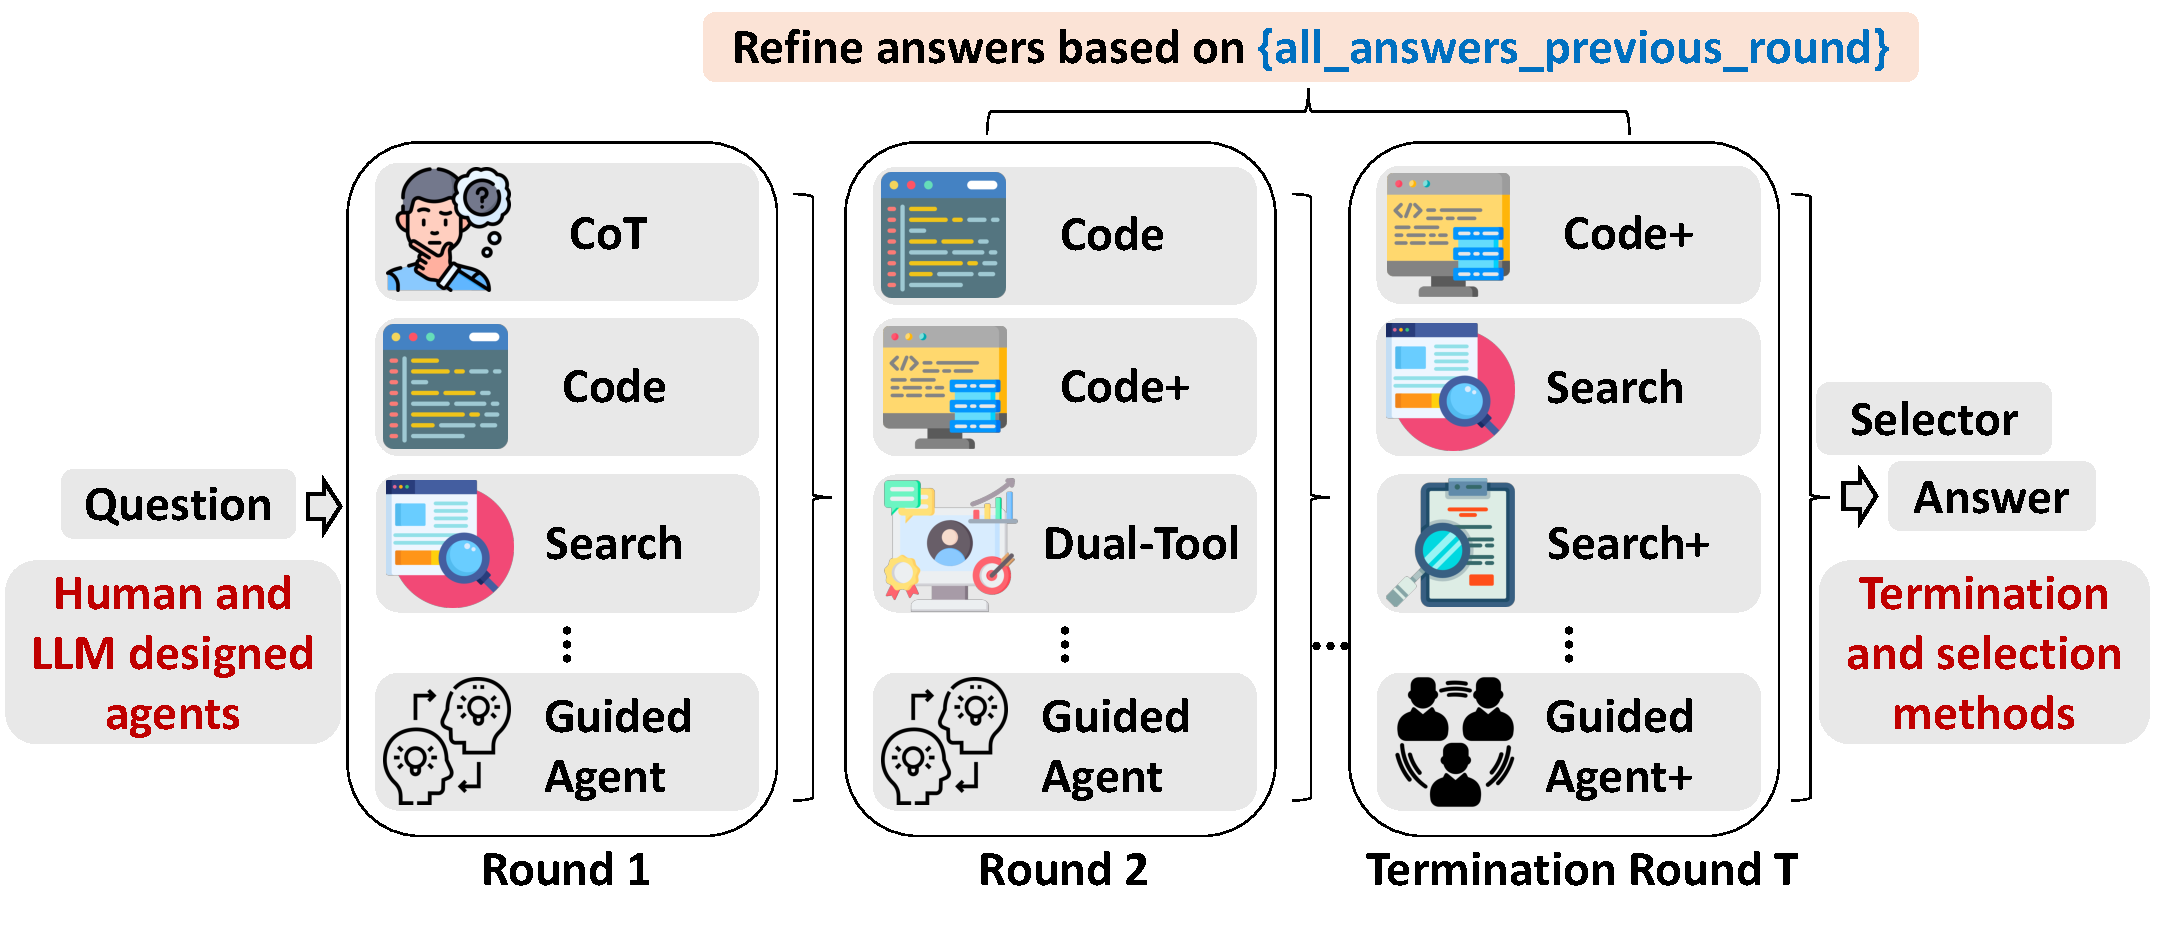
\includegraphics[width=0.95\linewidth]{Figures/Method.pdf}
   \caption{Overview of \texttt{TUMIX} framework. At each iteration, the responses from all agents in the previous round are concatenated with the original question, forming a joint prompt for the next round. This prompt is then provided to all agents (either the same or new agent groups) to produce refined answers. The subsequent prompts follow the structure illustrated in the above. The design of the agents, their number and specialization, the refinement termination criteria, and the selection strategies are the key factors that determine the effectiveness of the framework.}
   \label{fig:method_TUMIX}
   \vspace{-6pt}
\end{figure*}

%\vspace{-2pt}
\subsection{Pre-designed diverse agents}
\label{subsection:Pre-designed diverse agents}
\vspace{-6pt}
\begin{table}[t]
\centering
\caption{15 pre-designed agents used in \texttt{TUMIX}.}
\label{tab:agent_variants}
\footnotesize
\setlength{\tabcolsep}{4pt}
\renewcommand{\arraystretch}{1.05}
\begin{tabular}{@{}llp{0.66\linewidth}@{}}
\hline
\textbf{Full Name} & \textbf{Short Name} & \textbf{Description (15 agents)} \\
\hline
\texttt{w/o TTS}   & \texttt{Base}         & Direct prompt. \\
\texttt{CoT Agent}        & \texttt{CoT}         & Chain-of-Thought prompt~\citep{CoT}. \\
\texttt{CoT-Code Agent}  & \texttt{CoT$_{\text{code}}$}       & CoT prompt to output code. \\
\texttt{Search Agent}     & \texttt{S} & Uses WebSearch (LLM inherent tool only). \\
\texttt{Code Agent}       & \texttt{C}            & Uses Code Interpreter (base version). \\
\texttt{Code Agent+}      & \texttt{C$^{+}$}      & Uses Code Interpreter (hinted version with extra human pre-designed priors). \\
\texttt{Dual-Tool Agent} & \texttt{CS}           & Uses Code Interpreter + WebSearch (with 3 search variants). \\
\texttt{Guided Agent}     & \texttt{CSG}          & Dual-Tool agent (\texttt{CS}) \textit{guided} by a steering module~\citep{codesteer} (with 3 search variants). \\
\texttt{Guided Agent+}    & \texttt{CSG$^{+}$}    & \textit{Guided} agent (\texttt{CSG}) with enhanced/hinted prompts (with 3 search variants). \\
\hline
\end{tabular}
\vspace{-2mm}
\end{table}

As shown in Fig.~\ref{fig:method_TUMIX}, we regard \texttt{TUMIX} as sequential decision-making under a compute budget with diverse and correlated experts (agents). 
Each round selects which agents to run, what they may read (communication policy), when to stop (optimal stopping), and how to aggregate (decision rule), trading off accuracy and cost. Let \(q\) be a task with unknown correct answer \(a^\star\) in answer space \(\mathcal{A}\). There is a pool of agents \(\mathcal{S}=\{s_1,\dots,s_K\}\). Agent \(s_i\) outputs an answer \(Y_i\in\mathcal{A}\) at cost \(c_i\) and has competence
% \begin{equation}
$
  p_i(q) \;=\; \Prb\{Y_i = a^\star \mid q\}.
$
% \end{equation}
Let \(Z_i=\ind{Y_i=a^\star}\) denote correctness indicators. Their dependencies (and hence ensemble diversity) are captured by a correlation or mutual-information structure over \(\{Z_i\}\).

A policy \(\pi\) (our focus) chooses in each round: (i) which agents to run, (ii) the communication graph (what each agent may read from prior rounds), (iii) the stopping rule, and (iv) the aggregation rule producing \(\hat a_\pi\).
A canonical objective is
\begin{equation}
  \max_{\pi}\ \Prb\{\hat a_\pi = a^\star\} \;-\; \lambda \cdot \mathrm{Cost}_\pi,
\end{equation}
where \(\lambda>0\) trades off compute and accuracy. In our work, the $\mathrm{Cost}_\pi$ is the total number of inference times and input and output tokens to generate the final answer. In the default \texttt{TUMIX} setting, we utilize the same 15 pre-designed agents in all answer refinement rounds. These 15 agents have distinct reasoning and tool-use strategies, as summarized in Table~\ref{tab:agent_variants}. Agents with search access have three search methods (Google Search API (\texttt{gs}), inherent LLM search function (\texttt{llm}), or their combination (\texttt{com})), yielding three variants per agent. For agents employing multi-round interactions with Search or Code Interpreter, the maximum tool interaction round number is set to 5. In Section~\ref{sec:Human pre-designed agents vs. LLM generated agents}, we discuss how to further query LLMs to automatically optimize and design more diverse agents to achieve better performance. We also compare with a dynamic setting where agent types vary across rounds.

\vspace{-6pt}
\subsection{Refinement as message passing (accuracy rises and diversity shrinks)}
\vspace{-6pt}
\begin{figure*}[ht]
  \centering
  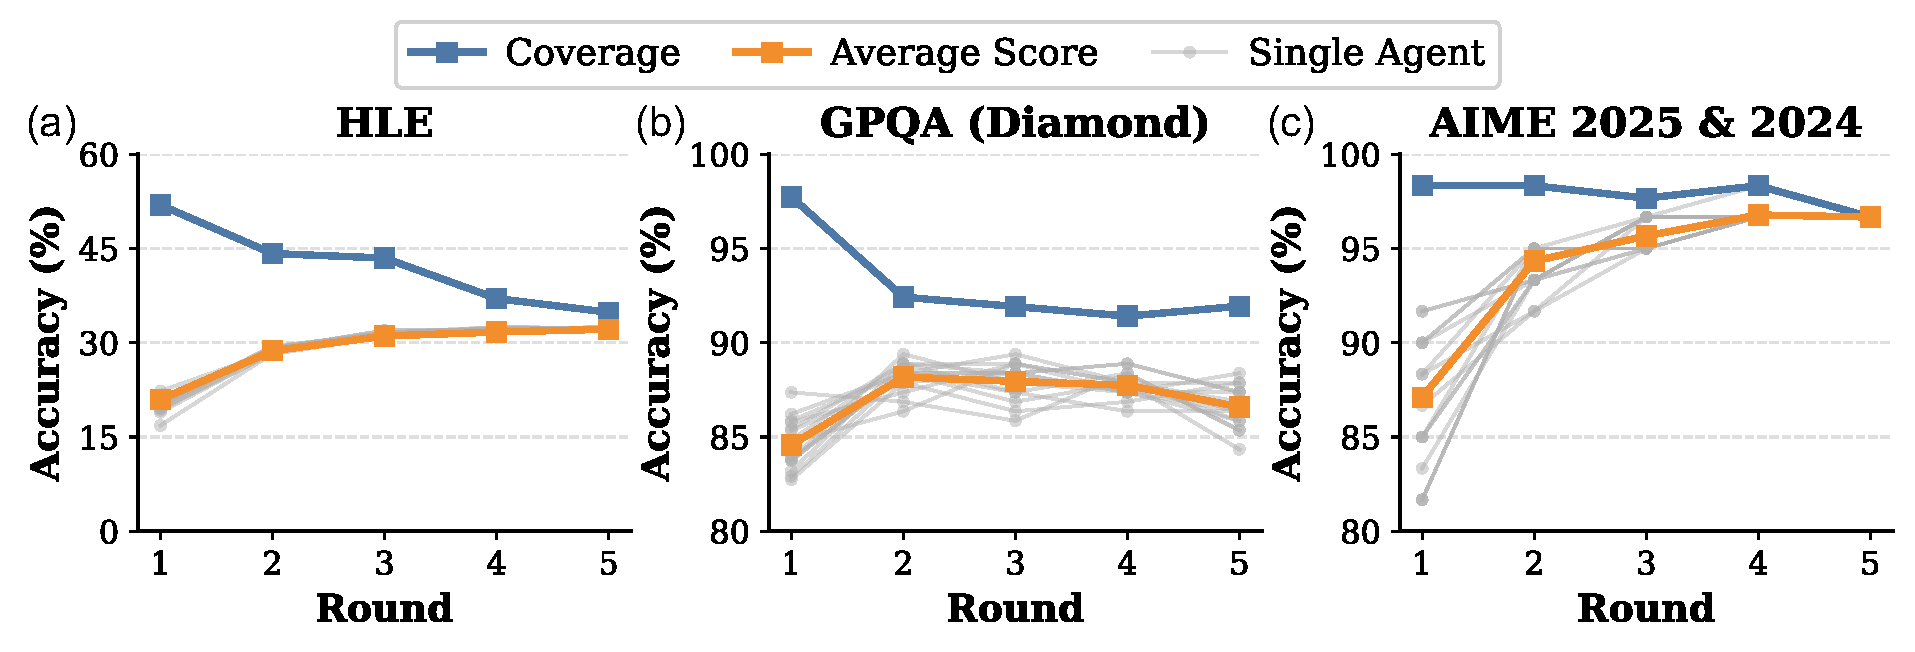
\includegraphics[width=0.9\linewidth]{Figures/acc_evolution_by_round.pdf}
  \vspace{-6pt}
   \caption{Evolution of coverage, individual agent scores, and average scores across refinement rounds. Coverage decreases monotonically across all benchmarks. For HLE and AIME, the average score rises over the initial rounds before plateauing. For GPQA, the average score improves early on but subsequently declines with further refinement.}
   \label{fig:acc_evolution_by_round}
   \vspace{-6pt}
\end{figure*}

\begin{figure*}[ht]
  \centering
  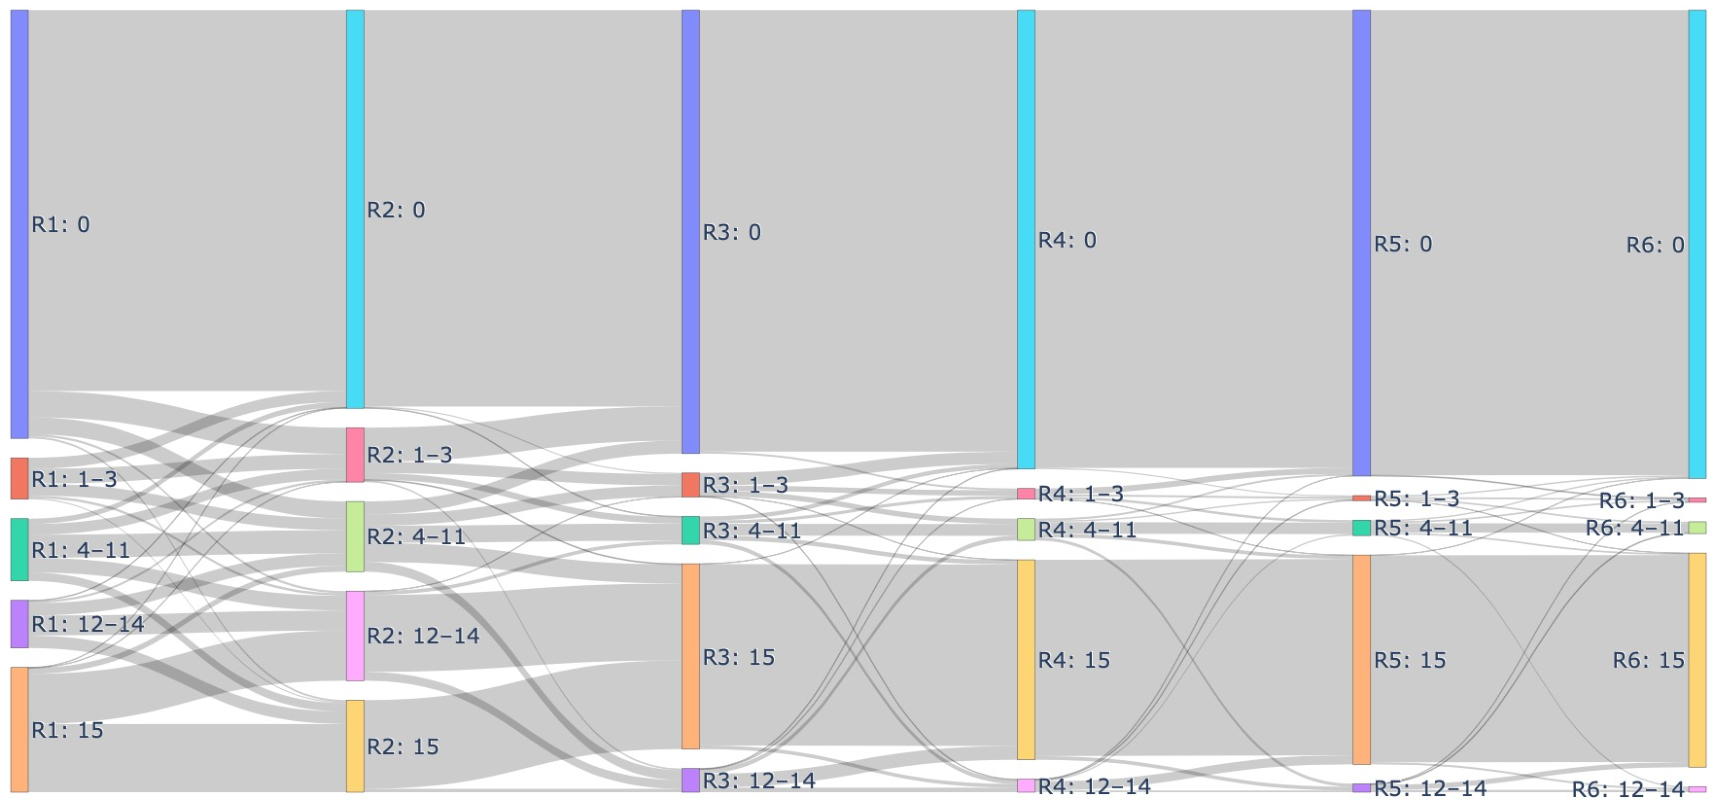
\includegraphics[width=0.9\linewidth]{Figures/sankey.pdf}
   \caption{Sankey diagram of the evolution of correctly answering agents across 2,500 HLE questions over refinement rounds. Based on the distribution dynamics, we define five categories: all wrong (0), few correct (1–3), moderate correct (4–11), high correct (12–14), and all correct (15).}
   \label{fig:sankey}
   \vspace{-12pt}
\end{figure*}

In each round, every agent independently generates a new solution by considering both the original question and the solutions provided by all agents in the previous round, as shown in Fig.~\ref{fig:method_TUMIX}. We evaluate the refinement process using two metrics: average accuracy and coverage (the probability of at least one correct) across agents in each round, which capture the quality and diversity of group answers~\citep{LLM-monkey}. For a set \(S\subseteq\mathcal{S}\), the coverage is
\begin{equation}
  Coverage(S) \;=\; \Prb\!\Big( \bigcup_{i\in S} \{Y_i = a^\star\} \Big).
\end{equation}
Under independence, \(Coverage(S) = 1-\prod_{i\in S}(1-p_i)\). With positive correlations, \(Coverage(S)\) shrinks. Fig.~\ref{fig:acc_evolution_by_round} shows the typical evolution dynamics of coverage, individual agent accuracy, and average scores over refinement rounds. Across all three benchmarks, coverage steadily declines, indicating that some correct answers are mistakenly discarded during iterative refinement. For HLE and AIME, the average score rises in the early rounds and then plateaus, while for GPQA it improves from round 1 to 2 but later declines. Fig.~\ref{fig:sankey} visualizes the dynamics over 2,500 HLE questions. From round 1 to 2, the number of partially correct cases (few/moderate/high correct) increases, while both all wrong and all correct cases decrease. This suggests that initial thought-sharing broadens exploration and promotes diversity. After round 2, however, partially correct cases diminish toward near zero, while all wrong and all correct cases grow. This indicates that agents gradually converge to a single shared answer across rounds, either correct or incorrect.

\vspace{-6pt}
\subsection{Termination in optimal rounds and final answer selection}
\label{subsection:Termination and selection}
\vspace{-6pt}
The observed evolution indicates that round-by-round refinement not only improves answers in the initial rounds but also drives convergence, as each agent selects based on prior responses. However, due to the limited reasoning ability of LLMs, many correct answers are prematurely discarded. Beyond the early rounds, refinement rarely yields further accuracy gains and, in some cases, even degrades performance. Thus, identifying an effective termination strategy is essential for both robust performance and cost efficiency. Let \(A_r\) denote acquired accuracy after round \(r\).
Define the expected marginal value of another round
\begin{equation}
  \Delta_r \;=\; \E\!\left[\, A_{r+1}-A_r \,\middle|\, \text{signals up to round } r \right].
\end{equation}
Stop at the first round \(r\) where \(\Delta_r \le \lambda \cdot \text{marginal cost (here is increased inference costs)}\).
A practical termination strategy decides whether to stop based on the estimated future gain $\Delta_r$, which relies on round-\(r\) statistics such as (i) diversity collapse (coverage drop; rising agreement), (ii) vote margin between top answers, and (iii) answer entropy.

In \texttt{TUMIX}, our termination determination strategy is to query the LLM to decide whether to stop refinement and finalize answers based on the current round, with a minimum round number of 2. We find this termination strategy achieves nearly the same performance with only 49\% of the inference cost. In Section~\ref{Sec: Experiments of Termination and selection methods}, we explore other termination methods such as stopping once the majority answer stabilizes across two consecutive rounds or termination based on LLM confidence scores~\citep{fu2025deep}, but find only worse performance. After termination, we obtain the final answer through majority voting over the agents’ responses, with Gemini-2.5-Pro selecting the most consistent output.